\documentclass[aspectratio=169]{beamer}
\usepackage{tikz}
\usepackage{graphicx}

\usecolortheme{whale}
\usetikzlibrary{er,positioning}  
\usetikzlibrary{decorations.pathreplacing}
\usetikzlibrary{arrows, decorations.markings}
\usetikzlibrary{shapes.geometric}

\setbeamertemplate{navigation symbols}{}

\definecolor{violet}{rgb}{0.53, 0.0, 0.69}

\definecolor{blue1}{RGB}{126,126,206}
\definecolor{blue2}{RGB}{87,87,192}
\definecolor{blue3}{RGB}{51,51,178}
\definecolor{blue4}{RGB}{27,26,107}

\tikzstyle{every link} = []
\tikzstyle{link} = [>=triangle 60, draw, every link]

\definecolor{attr}{RGB}{10,153,2}

\title{Bases de Datos I}
\subtitle{Modelo relacional: dise\~no intuitivo y lenguajes de consulta}
\author[Garc\'ia L., Cardentey V. M.]{
    Lic. V\'ictor M. Cardentey Fundora\\ 
    Dra. Lucina Garc\'ia Hern\'andez
}
\institute[MATCOM-UH]{
    Departamento de Computaci\'on\\
    Facultad de Matem\'atica y Computaci\'on\\
    Universidad de La Habana
}
\date[]{13 marzo de 2023}


\begin{document}
    \maketitle
    \begin{frame}{¿Hasta d\'onde hemos llegado?}
    \centering
    \resizebox{14cm}{7.5cm}{
    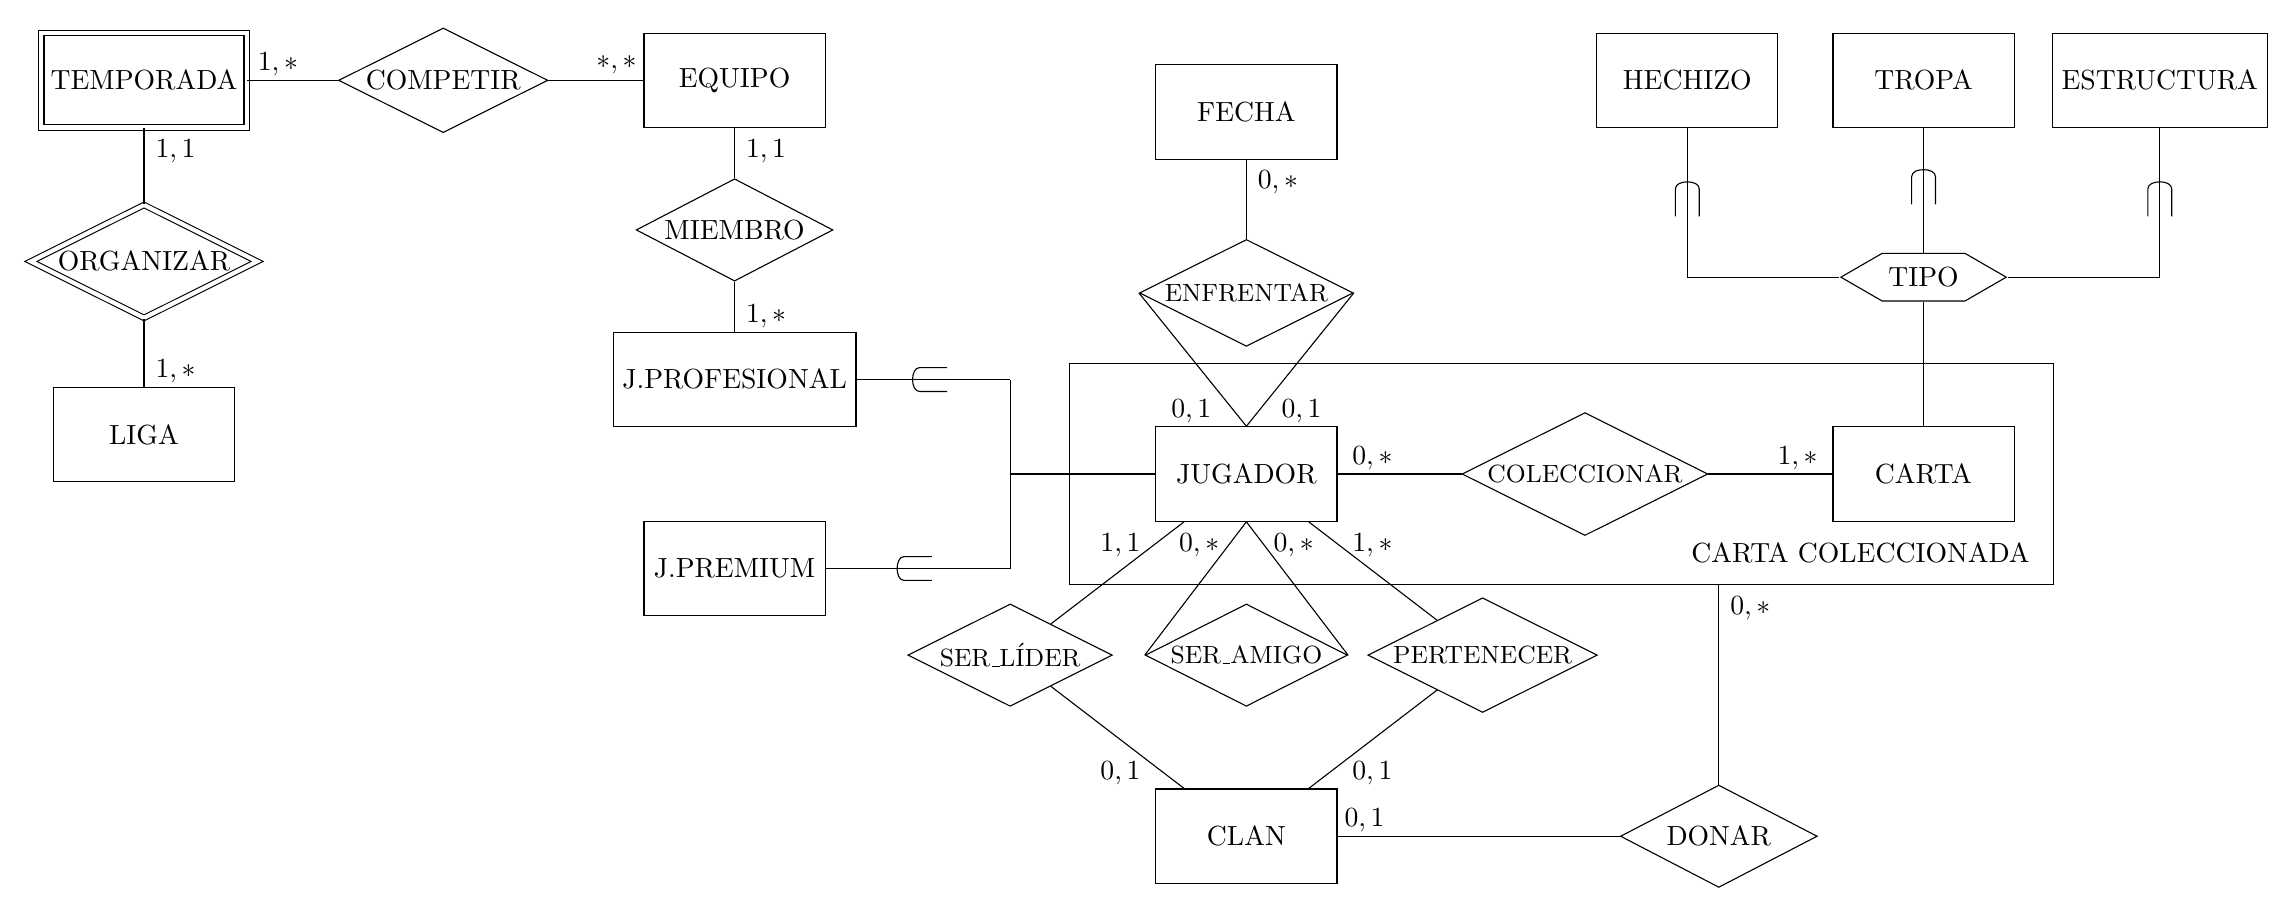
\begin{tikzpicture}
        \tikzstyle{every entity} = [minimum width=2.3cm, minimum height=1.2cm]
        \tikzstyle{every relationship} = [minimum width=2.5cm, minimum height=1.3cm]
        \tikzset{link/.append style={
            postaction={decorate},
            decoration={
                markings,
                mark= at position 0.5 with {
                    \draw (0.5em,1ex) -- (-0.5em,1ex) to[bend right=90] (-0.5em,-1ex) -- (0.5em,-1ex);
                }
            }
        }}
        \node[entity] (jugador) at (0,0) {JUGADOR};
        \node[entity] (fecha) at (0,4.6) {FECHA};
        \node[entity] (clan) at (0,-4.6) {CLAN};
        \node[entity] (carta) at (8.6,0) {CARTA};

        

        \node[entity] (tropa) at (8.6, 5) {TROPA};
        \node[entity] (estructura) at (11.6,5) {ESTRUCTURA};
        \node[entity] (hechizo) at (5.6,5) {HECHIZO};

        \node[regular polygon, draw, regular polygon sides=6, minimum width=7mm, xscale=3, label=center:TIPO] (tipo) at (8.6,2.5) {};
        \draw (carta.north) -- (tipo.south);
        \draw (tipo.west) -- (5.6,2.5);
        \draw (tipo.east) -- (11.6,2.5);
        \draw[link] (tropa.south) -- (tipo.north);
        \draw[link] (hechizo.south) -- (5.6,2.5);
        \draw[link] (estructura.south) -- (11.6,2.5);


        \node[relationship,aspect=2] (pertenecer) at (3,-2.3) {\small PERTENECER}
            edge(jugador) edge(clan);
        \node at (1.6,-0.9) {$1,\ast$};
        \node at (1.6,-3.8) {$0,1$};

        \node at (1.5,-4.4) {$0,1$};
        \node at (6.4,-1.7) {$0,\ast$};

        \node at (0.6,-0.9) {$0,\ast$};
        \node at (-0.6,-0.9) {$0,\ast$};

        \node[relationship,aspect=2] (coleccionar) at (4.3,0) {\small COLECCIONAR}
            edge(carta) edge(jugador);
        \node at (1.6,0.2) {$0,\ast$};
        \node at (7.0,0.2) {$1,\ast$};

        \node[relationship,aspect=2] (enfrentar) at (0,2.3) {\small ENFRENTAR}
            edge(fecha);
        \draw (enfrentar.west) -- (jugador.north);
        \draw (enfrentar.east) -- (jugador.north);
        \node at (0.7,0.8) {$0,1$};
        \node at (-0.7,0.8) {$0,1$};
        \node at (0.4,3.7) {$0,\ast$};

        \node[relationship,aspect=2] (seramigo) at (0, -2.3) {\small SER\_AMIGO};
        \draw (seramigo.east) -- (jugador.south);
        \draw (seramigo.west) -- (jugador.south);

        \node[relationship,aspect=2] (serlider) at (-3,-2.3) {\small SER\_L\'IDER}
            edge(jugador) edge(clan);
        \node at (-1.6,-3.8) {$0,1$};
        \node at (-1.6,-0.9) {$1,1$};

        \node[rectangle, draw, minimum width=12.5cm, minimum height=2.8cm] at (4,0) {};
        \node at (7.8,-1) {CARTA COLECCIONADA};

        \node[relationship, aspect=2] (donar) at (6,-4.6) {DONAR} edge(clan);
        \draw (6,-1.4) -- (donar.north);

        
        \draw (-3,0) -- (jugador.west);
        
        \node[entity] (premium) at (-6.5,-1.2) {J.PREMIUM};
        \node[entity] (profesional) at (-6.5,1.2) {J.PROFESIONAL};
        \draw (-3,0) -- (-3,-1.2);
        \draw (-3,0) -- (-3,1.2);
        \draw[link] (premium.east) -- (-3,-1.2);
        \draw[link] (profesional.east) -- (-3,1.2);


        \node[entity] (equipo) at (-6.5,5) {EQUIPO};
        \node at (-6.1,4.1) {$1,1$};
        \node at (-6.1,2) {$1,\ast$};

        \node[relationship,aspect=2] (miembro) at (-6.5,3.1) {MIEMBRO} edge(profesional) edge(equipo); 

        \node[entity,double distance=1.5pt] (temporada) at (-14, 5) {TEMPORADA};


        \node[entity] (liga) at (-14,0.5) {LIGA};
        \node[relationship,aspect=2,double distance=1.5pt] (organizar) at (-14,2.7) {ORGANIZAR} edge(temporada) edge(liga);

        \node[relationship,aspect=2] (compet) at (-10.2,5) {COMPETIR} edge(temporada) edge(equipo);
        
        \node at (-8,5.2) {$\ast,\ast$};
        \node at (-12.3,5.2) {$1,\ast$};

        \node at (-13.6,4.1) {$1,1$};
        \node at (-13.6,1.3) {$1,\ast$};
       
        



        
    \end{tikzpicture}
    }
\end{frame}

\begin{frame}{¿De d\'onde partimos?}
    \centering
    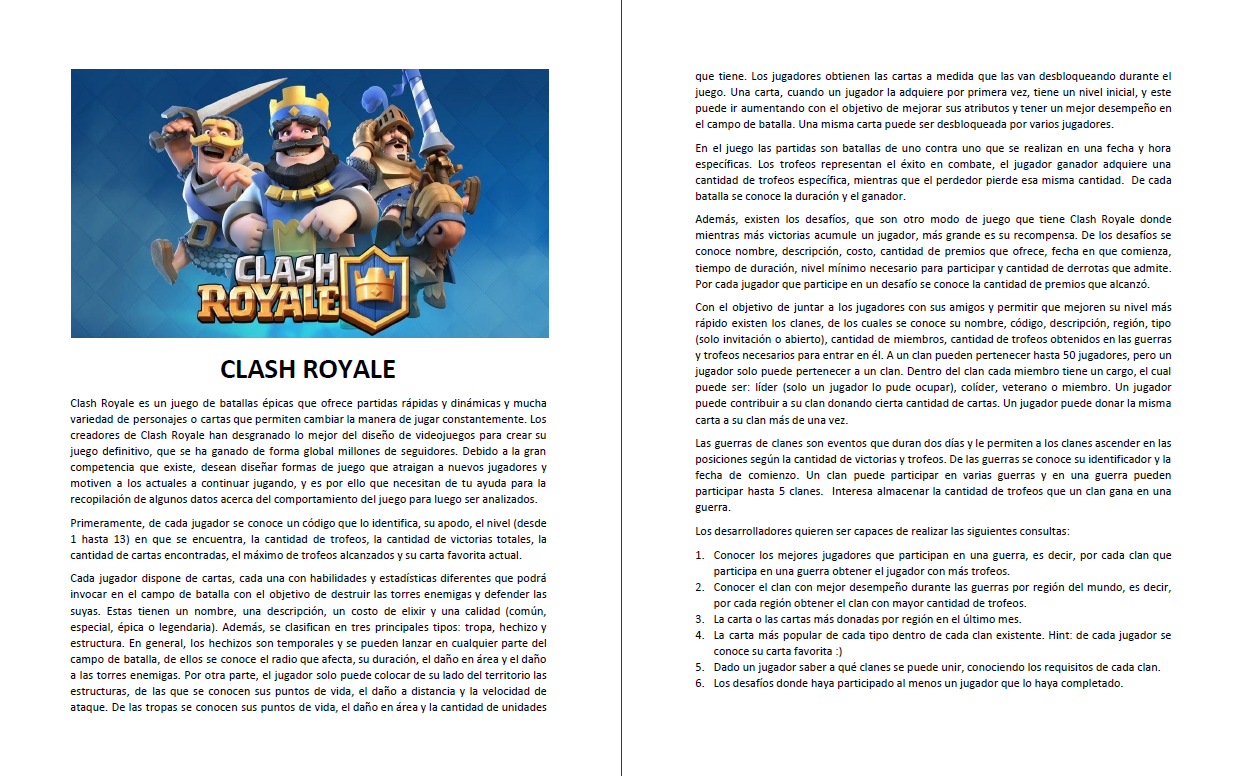
\includegraphics[width=0.8\linewidth, height=0.8\textheight]{img/specs.png}
\end{frame}

\begin{frame}{¿C\'omo obtener una especificaci\'on?}
    \begin{block}{An\'alisis de requerimientos}
        \begin{itemize}
            \item Descripciones en lenguaje natural
            \item Encuestas
            \item Observaci\'on directa 
            \item Formatos de registros
            \item Esquemas de datos
        \end{itemize}
    \end{block}
\end{frame}
    \begin{frame}{¿Para qu\'e est\'an aqu\'i?}
    \begin{block}{Objetivos para la conferencia}
        \begin{enumerate}
            \item Poder transformar un dise\~no conceptual descrito por el modelo MERX en un
            dise\~no l\'ogico basado en el modelo Relacional.
            \item Poder utilizar el dise\~no l\'ogico obtenido para responder las preguntas
            del usuario. 
        \end{enumerate}
        
    \end{block}
\end{frame}
    \begin{frame}{Transformando el dise\~no}
    \centering
    \Huge \textcolor{blue3}{Dise\~no intuitivo}
\end{frame}

{
\setbeamertemplate{background} 
{
    
\includegraphics[width=\paperwidth,height=\paperheight]{img/algorithm.jpg}
}
\begin{frame}
\end{frame}
}


\begin{frame}{Ahora s\'i... transformando el dise\~no}
    \centering
    \Huge \textcolor{blue3}{Algoritmo del dise\~no intuitivo}
\end{frame}


\begin{frame}{Dise\~no intuitivo}
    \begin{block}<2->{La idea b\'asica}
        
        \begin{enumerate}
            \item<2-> Convertir cada conjunto de entidades en una relaci\'on con el mismo conjunto de atributos.
            
            \item<4-> Convertir cada interrelaci\'on en una relaci\'on cuyos atributos son las llaves primarias de las
            relaciones que representan los conjuntos de entidades conectados.
        \end{enumerate}
    \end{block}
    

    \begin{columns}[T]
        \begin{column}{0.48\linewidth}

            \resizebox{\linewidth}{!}{
                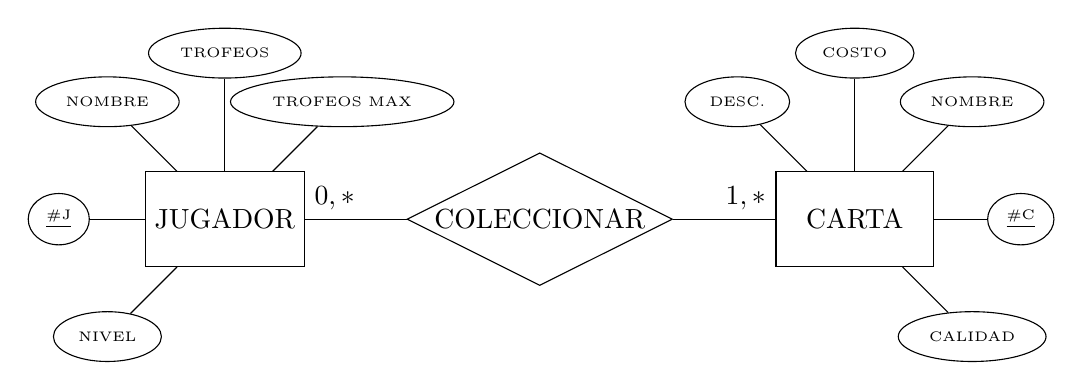
\begin{tikzpicture}[node distance=6em]
                    \tikzstyle{every entity} = [minimum width=2cm, minimum height=1.2cm]
                    \node[entity] (jugador) {JUGADOR}
                        [sibling distance=3cm]
                        child {node[attribute] [above right of=jugador] {\tiny TROFEOS MAX}}
                        child {node[attribute] [above of=jugador] {\tiny TROFEOS}}
                        child {node[attribute] [above left of=jugador] {\tiny NOMBRE}}
                        child {node[attribute] [left of=jugador] {\underline{\tiny \#J}}}
                        child {node[attribute] [below left of=jugador] {\tiny NIVEL}}
                        ;
                  
                    \node[entity] (clan) at (8,0) {CARTA}
                    [sibling distance=3cm]
                    child {node[attribute] [right of=clan] {\underline{\tiny \#C}}}
                    child {node[attribute] [above of=clan] {\tiny COSTO}}
                    child {node[attribute] [above left of=clan] {\tiny DESC.}}
                    child {node[attribute] [above right of=clan] {\tiny NOMBRE}}
                    child {node[attribute] [below right of=clan] {\tiny CALIDAD}};
                    
                  
                    \node[relationship,aspect=2] (pertenecer) at (4,0) {COLECCIONAR};
                    \draw (pertenecer.east) -- (clan.west) node[above left] {$1,\ast$};
                    \draw (pertenecer.west) -- (jugador.east) node[above right] {$0,\ast$};
                \end{tikzpicture}
            }
        \end{column}

        \begin{column}{0.48\linewidth}

        

                \begin{scriptsize}
                    \onslide<3->{
                        \textbf{Jugador}(\underline{\#J}, Nombre, Nivel, Trofeos, TrofeosMax)\\[2mm]
                        \textbf{Carta}(\underline{\#C}, Nombre, Calidad, Desc., Costo)\\[2mm]
                    }
                    \onslide<5->{
                        \textbf{Coleccionar}(\underline{\#J}, \underline{\#C})\\[1mm]
                        \hspace{4mm} FK: \#J REFERENCES Jugador\\
                        \hspace{4mm} FK: \#C REFERENCES Carta
                    }

                \end{scriptsize}

        \end{column}
        
    \end{columns}
\end{frame}



\begin{frame}{Aplicando el algoritmo}

    \begin{columns}[T]
        \begin{column}{0.48\linewidth}
            \centering
            \resizebox{\linewidth}{!}{
                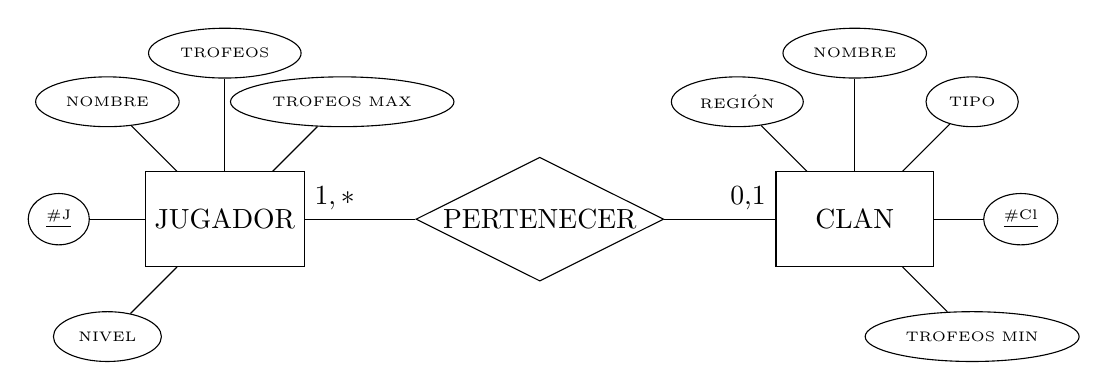
\begin{tikzpicture}[node distance=6em]
                    \tikzstyle{every entity} = [minimum width=2cm, minimum height=1.2cm]
                    \node[entity] (jugador) {JUGADOR}
                        [sibling distance=3cm]
                        child {node[attribute] [above right of=jugador] {\tiny TROFEOS MAX}}
                        child {node[attribute] [above of=jugador] {\tiny TROFEOS}}
                        child {node[attribute] [above left of=jugador] {\tiny NOMBRE}}
                        child {node[attribute] [left of=jugador] {\underline{\tiny \#J}}}
                        child {node[attribute] [below left of=jugador] {\tiny NIVEL}}
                        ;
                  
                    \node[entity] (clan) at (8,0) {CLAN}
                    [sibling distance=3cm]
                    child {node[attribute] [right of=clan] {\underline{\tiny \#Cl}}}
                    child {node[attribute] [above of=clan] {\tiny NOMBRE}}
                    child {node[attribute] [above left of=clan] {\tiny REGI\'ON}}
                    child {node[attribute] [above right of=clan] {\tiny TIPO}}
                    child {node[attribute] [below right of=clan] {\tiny TROFEOS MIN}};
                    
                  
                    \node[relationship,aspect=2] (pertenecer) at (4,0) {PERTENECER};
                    \draw (pertenecer.east) -- (clan.west) node[above left] {0,1};
                    \draw (pertenecer.west) -- (jugador.east)  node[above right] {$1, \ast$}; 
                \end{tikzpicture}
            }
        
        \end{column}

        \begin{column}{0.50\linewidth}
            \begin{scriptsize}
                \only<2-3>{
                    \textbf{Jugador}(\underline{\#J}, Nombre, Nivel, Trofeos, TrofeosMax)\\[2mm]
                    \textbf{Clan}(\underline{\#Cl}, Nombre, Regi\'on, Tipo, TrofeosMin)\\[2mm]
      
                    \textbf{Pertenecer}(\underline{\#J}, \underline{\#Cl})\\[1mm]
                    \hspace{4mm} FK: \#J REFERENCES Jugador\\[1mm]
                    \hspace{4mm} FK: \#Cl REFERENCES Clan
                }

        
            \end{scriptsize}
        \end{column}
        
    \end{columns}
   
    \vspace{10mm}
    \onslide<3>{
        \centering
        \textcolor{red}{\Large ¿Este dise\~no es eficiente?}


    }

    

\end{frame}


\begin{frame}{Un caso especial}

    \begin{columns}[T]
        \begin{column}{0.48\linewidth}
            \centering
            \resizebox{\linewidth}{!}{
                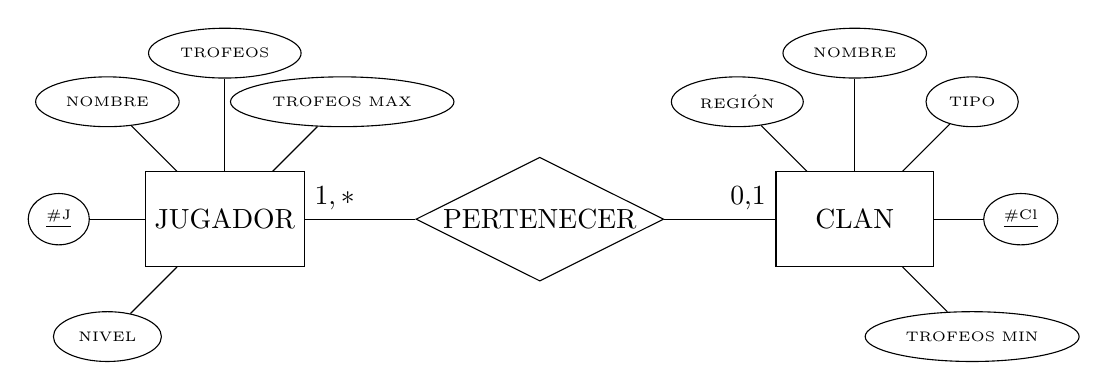
\begin{tikzpicture}[node distance=6em]
                    \tikzstyle{every entity} = [minimum width=2cm, minimum height=1.2cm]
                    \node[entity] (jugador) {JUGADOR}
                        [sibling distance=3cm]
                        child {node[attribute] [above right of=jugador] {\tiny TROFEOS MAX}}
                        child {node[attribute] [above of=jugador] {\tiny TROFEOS}}
                        child {node[attribute] [above left of=jugador] {\tiny NOMBRE}}
                        child {node[attribute] [left of=jugador] {\underline{\tiny \#J}}}
                        child {node[attribute] [below left of=jugador] {\tiny NIVEL}}
                        ;
                  
                    \node[entity] (clan) at (8,0) {CLAN}
                    [sibling distance=3cm]
                    child {node[attribute] [right of=clan] {\underline{\tiny \#Cl}}}
                    child {node[attribute] [above of=clan] {\tiny NOMBRE}}
                    child {node[attribute] [above left of=clan] {\tiny REGI\'ON}}
                    child {node[attribute] [above right of=clan] {\tiny TIPO}}
                    child {node[attribute] [below right of=clan] {\tiny TROFEOS MIN}};
                    
                  
                    \node[relationship,aspect=2] (pertenecer) at (4,0) {PERTENECER};
                    \draw (pertenecer.east) -- (clan.west) node[above left] {0,1};
                    \draw (pertenecer.west) -- (jugador.east)  node[above right] {$1, \ast$}; 
                \end{tikzpicture}
            }
        
        \end{column}

        \begin{column}{0.50\linewidth}
            \begin{scriptsize}


               
                    \vspace{5mm}
                    \textbf{Jugador}(\underline{\#J}, Nombre, Nivel, Trofeos, TrofeosMax, \#Cl)\\[1mm]
                    \hspace{4mm} FK: \#Cl REFERENCES Clan HAS NULL\\[2mm]
                    \textbf{Clan}(\underline{\#Cl}, Nombre, Regi\'on, Tipo, TrofeosMin)\\[2mm]
              
        
            \end{scriptsize}
        \end{column}
        
    \end{columns}
   
    \vspace{10mm}
    A\~nadir la llave primaria de la relaci\'on correspondiente al conjunto de entidades en el extremo con cardinalidad
            m\'axima \textcolor{red}{uno}
            a la relaci\'on correspondiente al conjunto de entidades en el otro extremo.
    

\end{frame}


\begin{frame}{Dise\~nos para interrelaciones de muchos a uno}
    \begin{columns}[T]
        \begin{column}{0.48\linewidth}
            \begin{scriptsize}
                \textbf{Jugador}(\underline{\#J}, Nombre, Nivel, Trofeos, TrofeosMax)\\[2mm]
                \textbf{Clan}(\underline{\#Cl}, Nombre, Regi\'on, Tipo, TrofeosMin)\\[2mm]
  
                \textbf{Pertenecer}(\underline{\#J}, \underline{\#Cl})\\[1mm]
                \hspace{4mm} FK: \#J REFERENCES Jugador\\
                \hspace{4mm} FK: \#Cl REFERENCES Clan
            \end{scriptsize}
        \end{column}

        \begin{column}{0.5\linewidth}
            \begin{scriptsize}
                \textbf{Jugador}(\underline{\#J}, Nombre, Nivel, Trofeos, TrofeosMax, \#Cl)\\[1mm]
                \hspace{4mm} FK: \#Cl REFERENCES Clan HAS NULL\\[2mm]
                \textbf{Clan}(\underline{\#Cl}, Nombre, Regi\'on, Tipo, TrofeosMin)\\[2mm]
            \end{scriptsize}
        \end{column}
        
    \end{columns}

    \vspace{5mm}

    \only<2>{
    \begin{center}
        \Large
        TAREA: ?`Cu\'ando uno es mejor que el otro?
    \end{center}
    }

    \note{@NOTE cu\'al es m\'as eficiente?}
\end{frame}

\begin{frame}{
    \only<1>{El caso especial del caso especial}
    \only<2>{Dise\~no para interrelaciones uno a uno: Opcionalidad}
    \only<3>{Dise\~no para interrelaciones uno a uno: Obligatoriedad}}

    \begin{columns}[T]
        \begin{column}{0.48\linewidth}
            \centering
            \resizebox{\linewidth}{!}{
                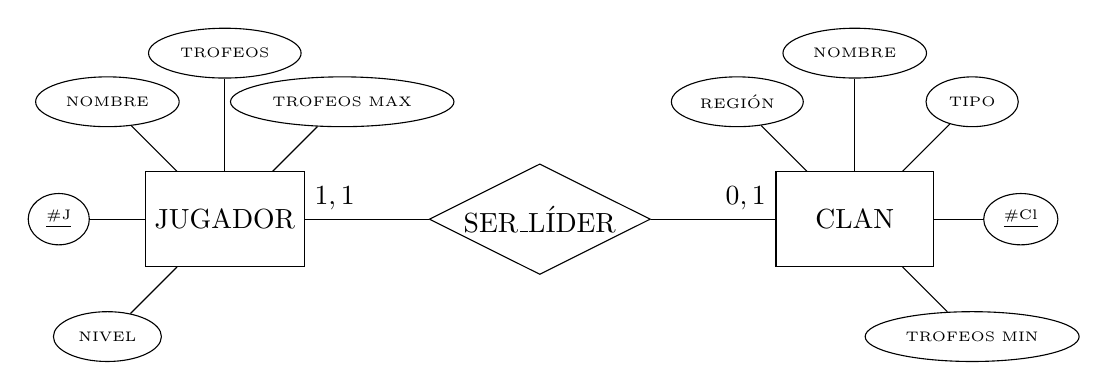
\begin{tikzpicture}[node distance=6em]
                    \tikzstyle{every entity} = [minimum width=2cm, minimum height=1.2cm]
                    \node[entity] (jugador) {JUGADOR}
                        [sibling distance=3cm]
                        child {node[attribute] [above right of=jugador] {\tiny TROFEOS MAX}}
                        child {node[attribute] [above of=jugador] {\tiny TROFEOS}}
                        child {node[attribute] [above left of=jugador] {\tiny NOMBRE}}
                        child {node[attribute] [left of=jugador] {\underline{\tiny \#J}}}
                        child {node[attribute] [below left of=jugador] {\tiny NIVEL}}
                        ;
                  
                    \node[entity] (clan) at (8,0) {CLAN}
                    [sibling distance=3cm]
                    child {node[attribute] [right of=clan] {\underline{\tiny \#Cl}}}
                    child {node[attribute] [above of=clan] {\tiny NOMBRE}}
                    child {node[attribute] [above left of=clan] {\tiny REGI\'ON}}
                    child {node[attribute] [above right of=clan] {\tiny TIPO}}
                    child {node[attribute] [below right of=clan] {\tiny TROFEOS MIN}};
                    
                  
                    \node[relationship,aspect=2] (pertenecer) at (4,0) {SER\_L\'IDER};
                    \draw (pertenecer.east) -- (clan.west) node[above left] {$0,1$};
                    \draw (pertenecer.west) -- (jugador.east)  node[above right] {$1, 1$}; 
                \end{tikzpicture}
            }
        
        \end{column}

        \begin{column}{0.50\linewidth}
            \begin{scriptsize}
                \only<2>{
                    \textbf{Jugador}(\underline{\#J}, Nombre, Nivel, Trofeos, TrofeosMax, \#Cl)\\[1mm]
                    \hspace{4mm} FK: \#Cl REFERENCES Clan HAS NULL\\[2mm]
                    \textbf{Clan}(\underline{\#Cl}, Nombre, Regi\'on, Tipo, TrofeosMin)\\[2mm]
                }

                \only<3>{
                    \vspace{5mm}
                    \textbf{Jugador}(\underline{\#J}, Nombre, Nivel, Trofeos, TrofeosMax)\\[1mm]
                    \textbf{Clan}(\underline{\#Cl}, Nombre, Regi\'on, Tipo, TrofeosMin, \#J)\\[1mm]
                    \hspace{4mm} FK: \#J REFERENCES Jugador\\[2mm]
                }
        
            \end{scriptsize}
        \end{column}

        
    \end{columns}
    
  
    

\end{frame}




\begin{frame}{Dise\~no para interrelaciones de uno a uno}

    \begin{columns}[T]
        \begin{column}{0.5\linewidth}
            \begin{scriptsize}
                
                \textbf{Jugador}(\underline{\#J}, Nombre, Nivel, Trofeos, TrofeosMax, \#Cl)\\[1mm]
                \hspace{4mm} FK: \#Cl REFERENCES Clan HAS NULL\\[2mm]
                \textbf{Clan}(\underline{\#Cl}, Nombre, Regi\'on, Tipo, TrofeosMin)\\[2mm]
            \end{scriptsize}
        \end{column}

        \begin{column}{0.48\linewidth}
            \begin{scriptsize}
                
                \textbf{Jugador}(\underline{\#J}, Nombre, Nivel, Trofeos, TrofeosMax)\\[1mm]
                \textbf{Clan}(\underline{\#Cl}, Nombre, Regi\'on, Tipo, TrofeosMin, \#J)\\[1mm]
                \hspace{4mm} FK: \#J REFERENCES Jugador\\[2mm]
            \end{scriptsize}
        \end{column}
        
    \end{columns}
    
    \vspace{5mm}

    \centering
    \large \textcolor{red}{Seleccionar el extremo con mayor cardinalidad m\'inima es m\'as eficiente}
    

\end{frame}


\begin{frame}{Dise\~no para interrelaciones con roles}
    \begin{columns}[T]

        \begin{column}{0.48\linewidth}
            \centering
            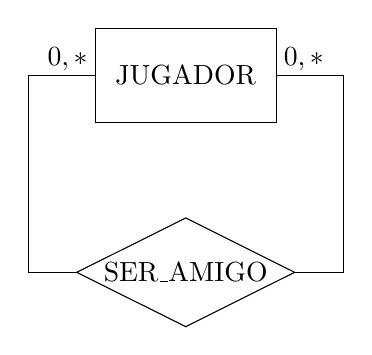
\begin{tikzpicture}
                \node[entity, minimum width=2.3cm, minimum height=1.2cm] (jugador) at (0,0) {JUGADOR};
                \node[relationship, aspect=2] (seramigo) at (0,-2.5) {SER\_AMIGO};
                \draw (seramigo.east) -- (2,-2.5) -- (2,0) -- (jugador.east);
                \draw (seramigo.west) -- (-2,-2.5) -- (-2,0) -- (jugador.west);
                \node at (-1.5,0.2) {$0 , \ast$};
                \node at (1.5,0.2) {$0,\ast$};
        
            \end{tikzpicture}
        \end{column}

        \begin{column}{0.48\linewidth}
            \vspace{15mm}
            \onslide<2->{

                \begin{scriptsize}
                    
                    \textbf{Ser\_Amigo}(\underline{\#Amigo1}, \underline{\#Amigo2})\\[1mm]
                    \hspace{4mm} FK: \#Amigo1 REFERENCES Jugador (\#J)\\[1mm]
                    \hspace{4mm} FK: \#Amigo2 REFERENCES Jugador (\#J)
                \end{scriptsize}
            }
        \end{column}
        
    \end{columns}
    \vspace{5mm}
    
    \onslide<3>{

        \centering
        \large \textcolor{red}{Se deben renombrar los atributos que tienen el mismo nombre}

    }

\end{frame}


\begin{frame}{Dise\~no para interrelaciones $n$-arias}
    \begin{columns}[T]
        \begin{column}{0.48\linewidth}
            \vspace{5mm}
            \centering
            \resizebox{\linewidth}{!}{
                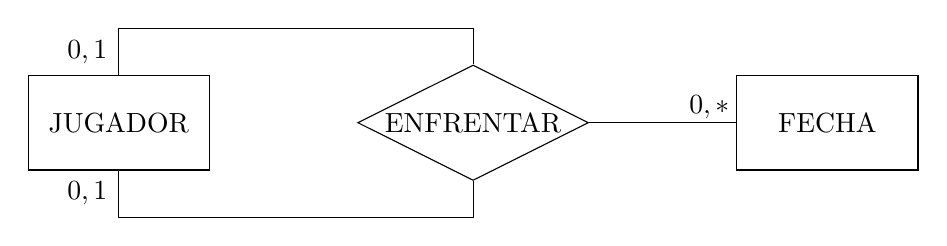
\begin{tikzpicture}
                    \tikzstyle{every entity} = [minimum width=2.3cm, minimum height=1.2cm]
                    \node[entity] (jugador) at (0,0) {JUGADOR};
                    \node[entity] (fecha) at (9,0) {FECHA};
                    \node[relationship, aspect=2] (enfrentar)at (4.5,0) {ENFRENTAR} edge(fecha);
                    \draw (jugador.south) -- (0,-1.2) -- (4.5,-1.2) -- (enfrentar.south); 
                    \draw (jugador.north) -- (0,1.2) -- (4.5,1.2) -- (enfrentar.north); 
            
                    \node at (-0.4,0.9) {$0,1$};
                    \node at (-0.4,-0.9) {$0,1$};
                    \node at (7.5,0.2) {$0,\ast$};
                \end{tikzpicture}
            }
        \end{column}

        \begin{column}{0.48\linewidth}
            \onslide<2->{

                \begin{scriptsize}
                    \textbf{Fecha}(\underline{Fecha})\\[2mm]
                    \textbf{Enfrentar}(\underline{\#J1}, \#J2, \underline{Fecha})\\[1mm]
                    \hspace{4mm}FK: \#J1 REFERENCES Jugador (\#J)\\[1mm]
                    \hspace{4mm}FK: \#J2 REFERENCES Jugador (\#J)\\[1mm]
                    \hspace{4mm}FK: Fecha REFERENCES Fecha\\[1mm]
                \end{scriptsize}
            }
        \end{column}
    \end{columns}
    
    \vspace{5mm}

    \onslide<3>{

        \begin{block}{}
            \begin{itemize}
                \item Convertir la interrelaci\'on en una relaci\'on cuyos atributos son las llaves primarias
                de las relaciones que representan los conjuntos de entidades conectados.
                \item   Si existen extremos
                de la interrelaci\'on con cardinalidad m\'axima uno, se escoge uno de ellos y su llave primaria
                se retira de la llave primaria de la relaci\'on resultante.
            \end{itemize}
        \end{block}
    }
        
     

   

   

\end{frame}

\begin{frame}{Dise\~no de agregaciones}
    \begin{columns}[T]
        \begin{column}{0.49\linewidth}
            \resizebox{\linewidth}{!}{
                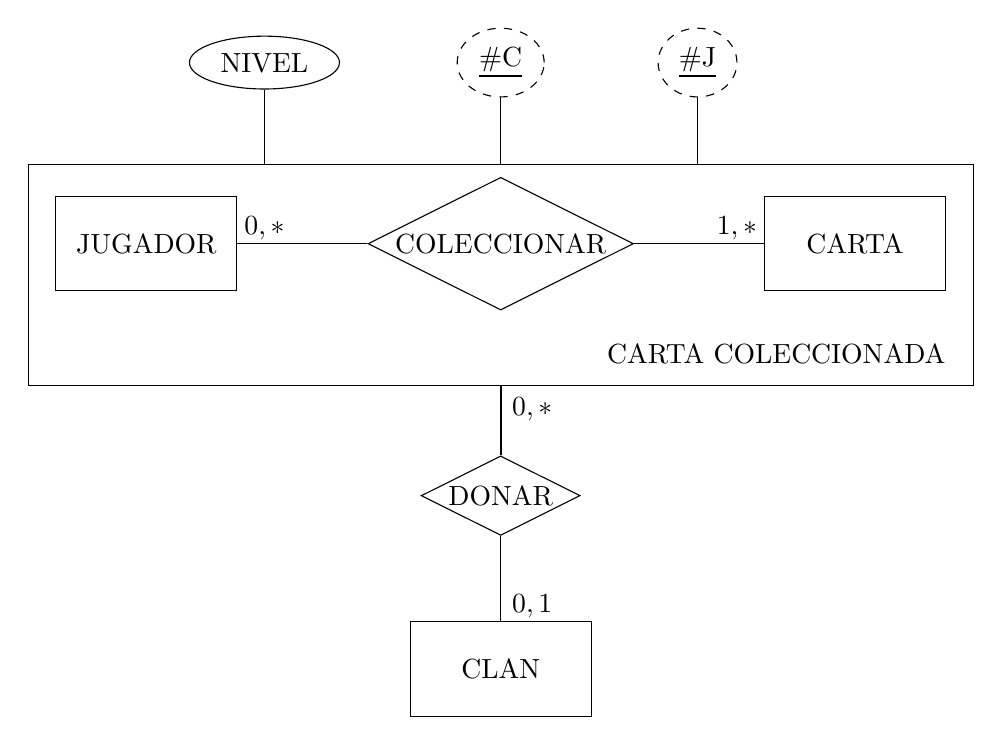
\begin{tikzpicture}
                    \tikzstyle{every entity} = [minimum width=2.3cm, minimum height=1.2cm]
                    \node[rectangle,draw,minimum width=12cm, minimum height=2.8cm] (coleccionada) at (4.5,-0.4) {};
                    \node[entity] (jugador) at (0,0) {JUGADOR};
                    \node[entity] (carta) at (9,0) {CARTA};
                    \node[relationship, aspect=2] (coleccionar) at (4.5,0) {COLECCIONAR} edge(jugador) edge(carta);
                    \node at (7.5,0.2) {$1,\ast$};
                    \node at (1.5,0.2) {$0,\ast$};
                    \node at (8,-1.4) {CARTA COLECCIONADA};
                    % \node[attribute] (nivel) at (4.5,2.3) { NIVEL};
                    % \draw[thick] (coleccionada.north) -- (nivel.south);

                    \node[entity] (clan) at (4.5,-5.4) {CLAN};
                    \node[relationship,aspect=2] (donar) at (4.5,-3.2) {DONAR} edge(clan);
                    \draw[thick] (coleccionada.south) -- (donar.north);
                    \node at (4.9, -2.1) {$0,\ast$};
                    \node at (4.9, -4.6) {$0,1$};

                    \node[attribute,dashed] (cartaid) at (4.5,2.3) { \underline{\#C}};
                    \node[attribute,dashed] (ci) at (7,2.3) {\underline{\#J}};
                    \node[attribute] (nivel) at (1.5,2.3) {NIVEL}; 
                    \draw (coleccionada.north) -- (cartaid.south);
                    \draw (7,1) -- (ci.south);
                    \draw (1.5,1) -- (nivel.south);
                \end{tikzpicture}
            }

        \end{column}

        \begin{column}{0.49\linewidth}
            \vspace{10mm}

            \onslide<2->{

                \begin{scriptsize}
                    
                    \textbf{Coleccionar}(\underline{\#J}, \underline{\#C}, \textcolor<3>{red}{Nivel})\\[2mm]
                    \textbf{Donar}(\underline{\#J}, \underline{\#C}, \underline{\#Cl})\\[1mm]
                    \hspace{2mm} FK: (\#J, \#C) REFERENCES Coleccionar (\#J, \#C)\\[1mm]
                    \hspace{2mm} FK: \#Cl REFERENCES Clan 
                    
                \end{scriptsize}
            }
        \end{column}
        
    \end{columns}
    \vspace{5mm}

    \onslide<3>{
        \centering
        \large \textcolor{red}{Agregar los atributos a la relaci\'on resultante de la interrelaci\'on}
        
    }
\end{frame}




\begin{frame}{Dise\~nos para la especializaci\'on}
    \begin{columns}[T]
        \begin{column}{0.40\linewidth}
            
            \centering
            \resizebox{\linewidth}{!}{
            \begin{tikzpicture}[node distance=5em]
                        \tikzset{link/.append style={
                    postaction={decorate},
                    decoration={
                        markings,
                        mark= at position 0.5 with {
                            \draw (0.5em,1ex) -- (-0.5em,1ex) to[bend right=90] (-0.5em,-1ex) -- (0.5em,-1ex);
                        }
                    }
                }}
                \tikzstyle{every entity} = [minimum width=2cm, minimum height=0.8cm]
        
                \node[entity] (jugador) {\small JUGADOR}
                    [sibling distance=3cm]
                    child {node[attribute] [above left of=jugador] {\tiny NIVEL}}
                    child {node[attribute] [above right of=jugador]{\tiny TROFEOS}}
                    child {node[attribute] [above of=jugador] {\tiny TROFEOS MAX}}
                    child {node[attribute] [right of=jugador]{\tiny NOMBRE}}
                    child {node[attribute] (ci) [left of=jugador] {\tiny \underline{\#J}}};
        
        
                \node[entity] (premium) at (-2,-3) {\small {\color<3->{blue}J. PREMIUM}}
                    [sibling distance=2.5cm]
                    child {node[attribute] [below left of=premium] {\tiny GASTO T.}}
                    child {node[attribute] [below right of=premium] {\tiny M. PAGO}}
                    child {node[attribute, dashed] [left of=premium] {\tiny \underline{\#J}}};
        
                \node[entity] (profesional) at (2,-3) {\small {\color<3->{orange}J. PROFESIONAL}}
                    [sibling distance=3.2cm]
                    child {node[attribute, dashed] [below left of=profesional] {\tiny \underline{\#J}}}
                    child {node[attribute] [below right of=profesional] {\tiny RANKING}};
        
                \draw[link] (premium.north) -- (-2,-1.3);
                \draw[link] (profesional.north) -- (2,-1.3);
                \draw (jugador.south) -- (0,-1.3);
                \draw (-2,-1.3) -- (0,-1.3);
                \draw (2,-1.3) -- (0,-1.3);
                % \draw[link] (premium.north) -- (jugador.south);
                % \draw[link] (profesional.north) -- (jugador.south);
        
                % \node[entity] (equipo) at (9,-3) {\small EQUIPO}
                % [sibling distance=3cm]
                % child {node[attribute] [above left of=equipo] {\tiny \underline{EQUIPO\_ID}}}
                % child {node[attribute] [above of=equipo] {\tiny NOMBRE}}
                % child {node[attribute] [above right of=equipo] {\tiny PA\'IS}};
                % \node[relationship, aspect=2] (miembro) at (5.8,-3) {\small MIEMBRO} edge(profesional) edge(equipo);
                % \node at (3.9,-2.8) {\small $1,\ast$};
                % \node at (7.6,-2.8) {\small $1,1$};
        
        
            \end{tikzpicture}
            }
        \end{column}

        \begin{column}{0.49\linewidth}
            \vspace{20mm}
            \onslide<2->{

                \begin{scriptsize}
                    
                    \textbf{Jugador}(\underline{\#J}, Nombre, Nivel, Trofeos, TrofeosMax, {\color<3->{blue}Gasto T.}, {\color<3->{blue}M. Pago}, {\color<3->{orange}Ranking})\\[2mm]
                \end{scriptsize}
            }
        \end{column}
        
    \end{columns}
    \vspace{5mm}

    \centering
    \onslide<4>{
        ¿Qu\'e ocurre si un jugador es profesional pero no premium?
    }
\end{frame}



\begin{frame}{Dise\~nos para la especializaci\'on}
    \begin{columns}[T]
        \begin{column}{0.40\linewidth}
            
            \centering
            \resizebox{\linewidth}{!}{
            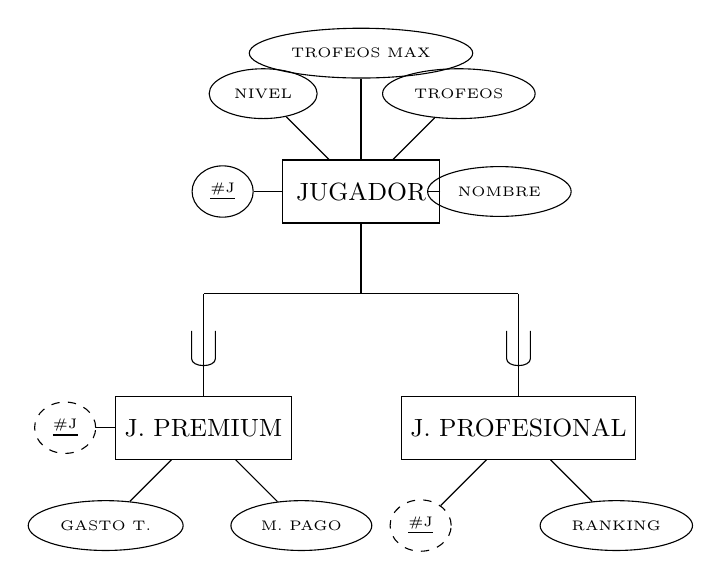
\begin{tikzpicture}[node distance=5em]
                        \tikzset{link/.append style={
                    postaction={decorate},
                    decoration={
                        markings,
                        mark= at position 0.5 with {
                            \draw (0.5em,1ex) -- (-0.5em,1ex) to[bend right=90] (-0.5em,-1ex) -- (0.5em,-1ex);
                        }
                    }
                }}
                \tikzstyle{every entity} = [minimum width=2cm, minimum height=0.8cm]
        
                \node[entity] (jugador) {\small JUGADOR}
                    [sibling distance=3cm]
                    child {node[attribute] [above left of=jugador] {\tiny NIVEL}}
                    child {node[attribute] [above right of=jugador]{\tiny TROFEOS}}
                    child {node[attribute] [above of=jugador] {\tiny TROFEOS MAX}}
                    child {node[attribute] [right of=jugador]{\tiny NOMBRE}}
                    child {node[attribute] (ci) [left of=jugador] {\tiny \underline{\#J}}};
        
        
                \node[entity] (premium) at (-2,-3) {\small J. PREMIUM}
                    [sibling distance=2.5cm]
                    child {node[attribute] [below left of=premium] {\tiny GASTO T.}}
                    child {node[attribute] [below right of=premium] {\tiny M. PAGO}}
                    child {node[attribute, dashed] [left of=premium] {\tiny \underline{\#J}}};
        
                \node[entity] (profesional) at (2,-3) {\small J. PROFESIONAL}
                    [sibling distance=3.2cm]
                    child {node[attribute, dashed] [below left of=profesional] {\tiny \underline{\#J}}}
                    child {node[attribute] [below right of=profesional] {\tiny RANKING}};
        
                \draw[link] (premium.north) -- (-2,-1.3);
                \draw[link] (profesional.north) -- (2,-1.3);
                \draw (jugador.south) -- (0,-1.3);
                \draw (-2,-1.3) -- (0,-1.3);
                \draw (2,-1.3) -- (0,-1.3);
                % \draw[link] (premium.north) -- (jugador.south);
                % \draw[link] (profesional.north) -- (jugador.south);
        
                % \node[entity] (equipo) at (9,-3) {\small EQUIPO}
                % [sibling distance=3cm]
                % child {node[attribute] [above left of=equipo] {\tiny \underline{EQUIPO\_ID}}}
                % child {node[attribute] [above of=equipo] {\tiny NOMBRE}}
                % child {node[attribute] [above right of=equipo] {\tiny PA\'IS}};
                % \node[relationship, aspect=2] (miembro) at (5.8,-3) {\small MIEMBRO} edge(profesional) edge(equipo);
                % \node at (3.9,-2.8) {\small $1,\ast$};
                % \node at (7.6,-2.8) {\small $1,1$};
        
        
            \end{tikzpicture}
            }
        \end{column}

        \begin{column}{0.49\linewidth}
            \vspace{15mm}
            \begin{scriptsize}
                
                \textbf{Jugador}(\underline{\#J}, Nombre, Nivel, Trofeos, TrofeosMax)\\[2mm]
                \textbf{J. Premium}(\underline{\#J}, Gasto T., M. Pago)\\[1mm]
                \hspace{4mm} FK: \#J REFERENCES Jugador\\[2mm]
                \textbf{J. Profesional}(\underline{\#J}, Ranking)\\[1mm]
                \hspace{4mm} FK: \#J REFERENCES Jugador
            \end{scriptsize}
        \end{column}
        
    \end{columns}
\end{frame}



\begin{frame}{Dise\~nos para la especializaci\'on}
    \begin{columns}[T]
        \begin{column}{0.48\linewidth}

            \begin{scriptsize}
                
                \textbf{Jugador}(\underline{\#J}, Nombre, Nivel, Trofeos, TrofeosMax, Gasto T., M. Pago, Ranking)\\[2mm]
            \end{scriptsize}
        \end{column}

        \begin{column}{0.48\linewidth}
            \begin{scriptsize}
                
                \textbf{Jugador}(\underline{\#J}, Nombre, Nivel, Trofeos, TrofeosMax)\\[2mm]
                \textbf{J. Premium}(\underline{\#J}, Gasto T., M. Pago)\\[1mm]
                \hspace{4mm} FK: \#J REFERENCES Jugador\\[2mm]
                \textbf{J. Profesional}(\underline{\#J}, Ranking)\\[1mm]
                \hspace{4mm} FK: \#J REFERENCES Jugador
            \end{scriptsize}
        \end{column}
        
    \end{columns}

    \note{@NOTE cu\'al es m\'as eficiente?}
\end{frame}



\begin{frame}{Dise\~nos para la especializaci\'on (partici\'on)}
    \begin{columns}[T]
        \begin{column}{0.48\linewidth}
            \resizebox{\linewidth}{!}{
    \begin{tikzpicture}[node distance=6em]
        \tikzset{link/.append style={
            postaction={decorate},
            decoration={
                markings,
                mark= at position 0.5 with {
                    \draw (0.5em,1ex) -- (-0.5em,1ex) to[bend right=90] (-0.5em,-1ex) -- (0.5em,-1ex);
                }
            }
        }}
        \tikzstyle{every entity} = [minimum width=2cm, minimum height=0.8cm]
        \node[entity] (carta) at (0,0) {CARTA}
        [sibling distance=3cm]
        child {node[attribute] [above left of=carta] {\tiny CALIDAD}}
        child {node[attribute] [above right of=carta]{\tiny DESC.}}
        child {node[attribute] [above of=carta] {\tiny NOMBRE}}
        child {node[attribute] [right of=carta]{\tiny COSTO}}
        child {node[attribute] [left of=carta] {\tiny \underline{CARTA\_ID}}};
        \node[regular polygon, draw, regular polygon sides=6, minimum width=7mm, xscale=3, label=center:TIPO] (tipo) at (0,-2) {};
        \draw (carta.south) -- (tipo.north);
        \node[entity] (tropa) at (0,-4.5) {{\color<2->{orange}TROPA}}
        [sibling distance=3cm]
        child {node[attribute, dashed] [above left of=tropa] {\tiny \underline{CARTA\_ID}}}
        child {node[attribute] [below of=tropa] {\tiny P. VIDA}}
        child {node[attribute] [below right of=tropa] {\tiny D. \'AREA}}
        child {node[attribute] [above right of=tropa] {\tiny UNIDADES}};
        \node[entity] (hechizo) at (-4,-4.5) {{\color<2->{blue}HECHIZO}}
        [sibling distance=3cm]
        child {node[attribute, dashed] [left of=hechizo] {\tiny \underline{CARTA\_ID}}}
        child {node[attribute] [below left of=hechizo] {\tiny RADIO}}
        child {node[attribute] [below of=hechizo] {\tiny DURACI\'ON}}
        child {node[attribute] [below right of=hechizo] {\tiny D. \'AREA}}
        child {node[attribute] [above left of=hechizo] {\tiny D. TORRES}};
        \node[entity] (estructura) at (3.4,-4.5) {{\color<2->{violet}ESTRUCTURA}}
        [sibling distance=3cm]
        child {node[attribute, dashed] [above right of=estructura] {\tiny \underline{CARTA\_ID}}}
        child {node[attribute] [right of=estructura] {\tiny D. DIST}}
        child {node[attribute] [below of=estructura] {\tiny V. ATAQUE}}
        child {node[attribute] [below right of=estructura] {\tiny P. VIDA}}
        ;
        \draw[link] (tropa.north) -- (tipo.south);
        \draw (-4,-2) -- (-1,-2);
        \draw[link] (hechizo.north) -- (-4,-2); 
        \draw (3.4,-2) -- (1,-2);
        \draw[link] (estructura.north) -- (3.4,-2);
    \end{tikzpicture}
    }
            
        \end{column}

        \begin{column}{0.48\linewidth}
            \vspace{20mm}

            \onslide<2->{

                \begin{scriptsize}
                    
                    \textbf{Carta}(\underline{\#C}, Nombre, Calidad, Desc., Costo, {\color<2->{blue}D.Torres}, {\color<2->{blue}Radio}, 
                    {\color<2->{blue}Duraci\'on}, {\color<2->{blue}H. D. \'Area}, {\color<2->{orange}Unidades}, {\color<2->{orange}T. P. Vida}, {\color<2->{orange}T. D. \'Area},
                    {\color<2->{violet}D. Dist}, {\color<2->{violet}E. P. Vida}, {\color<2->{violet}V. Ataque})
                \end{scriptsize}
            }
        \end{column}
        
    \end{columns}
    \vspace{5mm}

    \onslide<3>{

        \centering
        \large \textcolor{red}{Muy ineficiente espacialmente}
    }

    \note<3>{@NOTE por qu\'e?}
\end{frame}



\begin{frame}{Dise\~nos para la especializaci\'on (partici\'on)}
    \begin{columns}[T]
        \begin{column}{0.48\linewidth}
            \resizebox{\linewidth}{!}{
    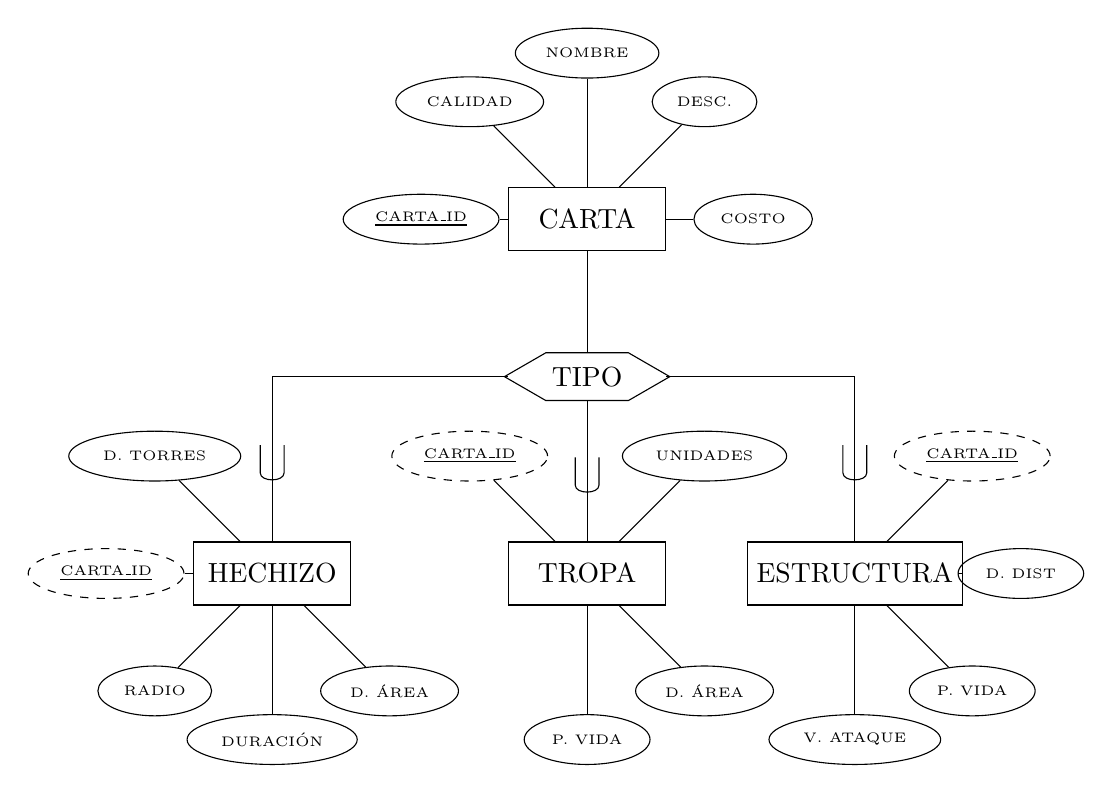
\begin{tikzpicture}[node distance=6em]
        \tikzset{link/.append style={
            postaction={decorate},
            decoration={
                markings,
                mark= at position 0.5 with {
                    \draw (0.5em,1ex) -- (-0.5em,1ex) to[bend right=90] (-0.5em,-1ex) -- (0.5em,-1ex);
                }
            }
        }}
        \tikzstyle{every entity} = [minimum width=2cm, minimum height=0.8cm]
        \node[entity] (carta) at (0,0) {CARTA}
        [sibling distance=3cm]
        child {node[attribute] [above left of=carta] {\tiny CALIDAD}}
        child {node[attribute] [above right of=carta]{\tiny DESC.}}
        child {node[attribute] [above of=carta] {\tiny NOMBRE}}
        child {node[attribute] [right of=carta]{\tiny COSTO}}
        child {node[attribute] [left of=carta] {\tiny \underline{CARTA\_ID}}};
        \node[regular polygon, draw, regular polygon sides=6, minimum width=7mm, xscale=3, label=center:TIPO] (tipo) at (0,-2) {};
        \draw (carta.south) -- (tipo.north);
        \node[entity] (tropa) at (0,-4.5) {TROPA}
        [sibling distance=3cm]
        child {node[attribute, dashed] [above left of=tropa] {\tiny \underline{CARTA\_ID}}}
        child {node[attribute] [below of=tropa] {\tiny P. VIDA}}
        child {node[attribute] [below right of=tropa] {\tiny D. \'AREA}}
        child {node[attribute] [above right of=tropa] {\tiny UNIDADES}};
        \node[entity] (hechizo) at (-4,-4.5) {HECHIZO}
        [sibling distance=3cm]
        child {node[attribute, dashed] [left of=hechizo] {\tiny \underline{CARTA\_ID}}}
        child {node[attribute] [below left of=hechizo] {\tiny RADIO}}
        child {node[attribute] [below of=hechizo] {\tiny DURACI\'ON}}
        child {node[attribute] [below right of=hechizo] {\tiny D. \'AREA}}
        child {node[attribute] [above left of=hechizo] {\tiny D. TORRES}};
        \node[entity] (estructura) at (3.4,-4.5) {ESTRUCTURA}
        [sibling distance=3cm]
        child {node[attribute, dashed] [above right of=estructura] {\tiny \underline{CARTA\_ID}}}
        child {node[attribute] [right of=estructura] {\tiny D. DIST}}
        child {node[attribute] [below of=estructura] {\tiny V. ATAQUE}}
        child {node[attribute] [below right of=estructura] {\tiny P. VIDA}}
        ;
        \draw[link] (tropa.north) -- (tipo.south);
        \draw (-4,-2) -- (-1,-2);
        \draw[link] (hechizo.north) -- (-4,-2); 
        \draw (3.4,-2) -- (1,-2);
        \draw[link] (estructura.north) -- (3.4,-2);
    \end{tikzpicture}
    }
            
        \end{column}

        \begin{column}{0.48\linewidth}
            \vspace{12mm}
            \begin{scriptsize}
                
                \textbf{Carta}(\underline{\#C}, Nombre, Calidad, Desc., Costo)\\[2mm]
                \textbf{Hechizo}(\underline{\#C}, D.Torres, Radio, Duraci\'on, D. \'Area)\\[1mm]
                \hspace{4mm} FK: \#C REFERENCES Carta \\[2mm]
                \textbf{Tropa}(\underline{\#C}, Unidades, P. Vida, D. \'Area)\\[1mm]
                \hspace{4mm} FK: \#C REFERENCES Carta \\[2mm]
                
                \textbf{Estructura}(\underline{\#C}, D. Dist, P. Vida, V. Ataque)\\[1mm]
                \hspace{4mm} FK: \#C REFERENCES Carta\\[2mm]
            \end{scriptsize}
        \end{column}
        
    \end{columns}


\end{frame}


\begin{frame}{Dise\~nos para la especializaci\'on (partici\'on)}
    \begin{columns}[T]
        \begin{column}{0.48\linewidth}
            \resizebox{\linewidth}{!}{
    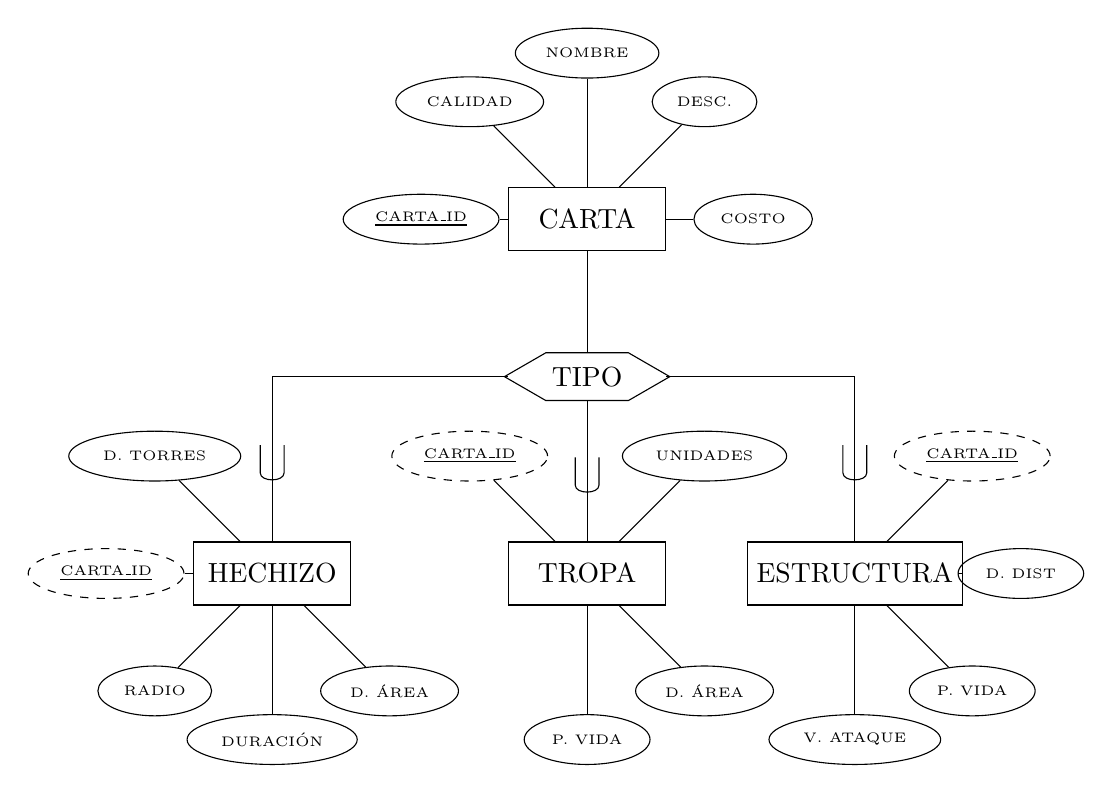
\begin{tikzpicture}[node distance=6em]
        \tikzset{link/.append style={
            postaction={decorate},
            decoration={
                markings,
                mark= at position 0.5 with {
                    \draw (0.5em,1ex) -- (-0.5em,1ex) to[bend right=90] (-0.5em,-1ex) -- (0.5em,-1ex);
                }
            }
        }}
        \tikzstyle{every entity} = [minimum width=2cm, minimum height=0.8cm]
        \node[entity] (carta) at (0,0) {CARTA}
        [sibling distance=3cm]
        child {node[attribute] [above left of=carta] {\tiny CALIDAD}}
        child {node[attribute] [above right of=carta]{\tiny DESC.}}
        child {node[attribute] [above of=carta] {\tiny NOMBRE}}
        child {node[attribute] [right of=carta]{\tiny COSTO}}
        child {node[attribute] [left of=carta] {\tiny \underline{CARTA\_ID}}};
        \node[regular polygon, draw, regular polygon sides=6, minimum width=7mm, xscale=3, label=center:TIPO] (tipo) at (0,-2) {};
        \draw (carta.south) -- (tipo.north);
        \node[entity] (tropa) at (0,-4.5) {TROPA}
        [sibling distance=3cm]
        child {node[attribute, dashed] [above left of=tropa] {\tiny \underline{CARTA\_ID}}}
        child {node[attribute] [below of=tropa] {\tiny P. VIDA}}
        child {node[attribute] [below right of=tropa] {\tiny D. \'AREA}}
        child {node[attribute] [above right of=tropa] {\tiny UNIDADES}};
        \node[entity] (hechizo) at (-4,-4.5) {HECHIZO}
        [sibling distance=3cm]
        child {node[attribute, dashed] [left of=hechizo] {\tiny \underline{CARTA\_ID}}}
        child {node[attribute] [below left of=hechizo] {\tiny RADIO}}
        child {node[attribute] [below of=hechizo] {\tiny DURACI\'ON}}
        child {node[attribute] [below right of=hechizo] {\tiny D. \'AREA}}
        child {node[attribute] [above left of=hechizo] {\tiny D. TORRES}};
        \node[entity] (estructura) at (3.4,-4.5) {ESTRUCTURA}
        [sibling distance=3cm]
        child {node[attribute, dashed] [above right of=estructura] {\tiny \underline{CARTA\_ID}}}
        child {node[attribute] [right of=estructura] {\tiny D. DIST}}
        child {node[attribute] [below of=estructura] {\tiny V. ATAQUE}}
        child {node[attribute] [below right of=estructura] {\tiny P. VIDA}}
        ;
        \draw[link] (tropa.north) -- (tipo.south);
        \draw (-4,-2) -- (-1,-2);
        \draw[link] (hechizo.north) -- (-4,-2); 
        \draw (3.4,-2) -- (1,-2);
        \draw[link] (estructura.north) -- (3.4,-2);
    \end{tikzpicture}
    }
            
        \end{column}

        \begin{column}{0.48\linewidth}
            \vspace{12mm}
            \begin{scriptsize}
                \textbf{Hechizo}(\underline{\#C}, Nombre, Calidad, Desc., Costo, D.Torres, Radio, Duraci\'on, D. \'Area)\\[1mm]
               
                \textbf{Tropa}(\underline{\#C}, Nombre, Calidad, Desc., Costo, Unidades, P. Vida, D. \'Area)\\[1mm]
                \textbf{Estructura}(\underline{\#C}, Nombre, Calidad, Desc., Costo, D. Dist, P. Vida, V. Ataque)\\[1mm]
            \end{scriptsize}
        \end{column}
        
    \end{columns}


\end{frame}


\begin{frame}{Dise\~nos para la especializaci\'on (partici\'on)}

    \begin{columns}[T]

        \begin{column}{0.48\linewidth}
            \begin{scriptsize}
                
                \textbf{Carta}(\underline{\#C}, Nombre, Calidad, Desc., Costo)\\[2mm]
                \textbf{Hechizo}(\underline{\#C}, D.Torres, Radio, Duraci\'on, D. \'Area)\\[1mm]
                \hspace{4mm} FK: \#C REFERENCES Carta \\[2mm]
                \textbf{Tropa}(\underline{\#C}, Unidades, P. Vida, D. \'Area)\\[1mm]
                \hspace{4mm} FK: \#C REFERENCES Carta \\[2mm]
                
                \textbf{Estructura}(\underline{\#C}, D. Dist, P. Vida, V. Ataque)\\[1mm]
                \hspace{4mm} FK: \#C REFERENCES Carta\\[2mm]
            \end{scriptsize}
        \end{column}

        \begin{column}{0.48\linewidth}

            \begin{scriptsize}
                \textbf{Hechizo}(\underline{\#C}, Nombre, Calidad, Desc., Costo, D.Torres, Radio, Duraci\'on, D. \'Area)\\[1mm]
               
                \textbf{Tropa}(\underline{\#C}, Nombre, Calidad, Desc., Costo, Unidades, P. Vida, D. \'Area)\\[1mm]
               
                \textbf{Estructura}(\underline{\#C}, Nombre, Calidad, Desc., Costo, D. Dist, P. Vida, V. Ataque)\\[1mm]
             
            \end{scriptsize}
        \end{column}
        
    \end{columns}

    \vspace{5mm}

    \only<2>{
    \begin{center}
        \Large
        TAREA: ?`Cu\'ando uno es mejor que el otro?
    \end{center}
    }

    \note{@NOTE cu\'al es m\'as eficiente?}
\end{frame}


\begin{frame}{Dise\~no para las entidades d\'ebiles}

    \begin{columns}[T]
        \begin{column}{0.48\linewidth}
            \centering
            \resizebox{!}{6cm}{
                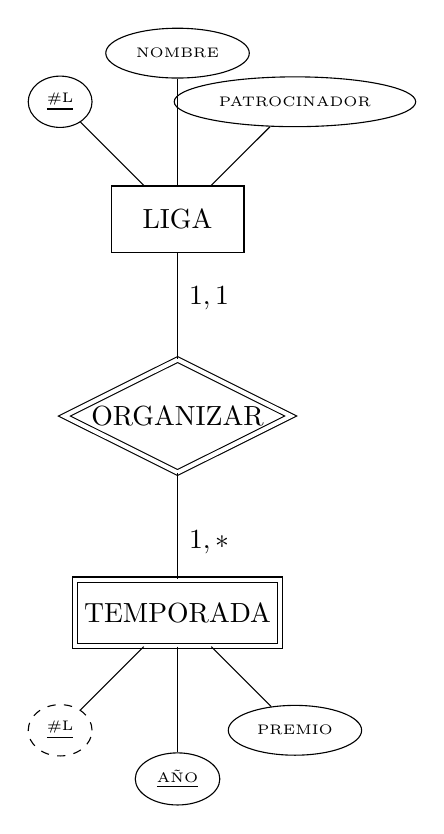
\begin{tikzpicture}[node distance=6em]
                    \node[entity] (liga) at (0,0) {LIGA}
                    [sibling distance=3cm]
                    child {node[attribute] [above of=liga] {\tiny NOMBRE}}
                    child {node[attribute] [above right of=liga] {\tiny PATROCINADOR}}
                    child {node[attribute] [above left of=liga] {\tiny \underline{\#L}} };
                    \node[entity,double distance =1.5 pt] (temp) at (0,-5) {TEMPORADA}
                    child {node[attribute,dashed] [below left of=temp] {\tiny \underline{\#L}} }
                    child {node[attribute] [below of =temp] {\underline{\tiny A\~NO}}}
                    child {node[attribute] [below right of=temp] {\tiny PREMIO}};
                  
                    \node[relationship,aspect=2,double distance =1.5 pt] (organizar) at (0,-2.5) {ORGANIZAR} edge(liga) edge(temp);

            
                    \node at (0.4,-1) {$1,1$};
                    \node at (0.4,-4.1) {$1,\ast$};
                  
                \end{tikzpicture}
                }
        \end{column}

        \begin{column}{0.48\linewidth}
            \vspace{20mm}

            \onslide<2->{

                \begin{scriptsize}
                    \textbf{Liga}(\underline{\#L}, Nombre, Patrocinador)\\[2mm]
    
                
                    \textbf{Temporada}(\underline{\#L}, \underline{A\~no}, Premio)\\[1mm]
                    \hspace{4mm} FK: \#L REFERENCES Liga
                \end{scriptsize}
            }
        \end{column}
    \end{columns}
\end{frame}


\begin{frame}{}
    \begin{columns}[T]
        \begin{column}{0.46\linewidth}
            \vspace{33mm}

            \Large \textcolor{blue3}{El dise\~no l\'ogico no es subjetivo}
        \end{column}

        \begin{column}{0.53\linewidth}
            
\includegraphics[width=\linewidth, height=0.8\textheight]{img/design.jpg}
        \end{column}
        
    \end{columns}
\end{frame}



% \begin{frame}{F\'acil}


% \end{frame}

    \begin{frame}{Respondiendo preguntas}

    \centering
    \Huge\textcolor{blue3}{Lenguajes de consulta}
    
\end{frame}


\begin{frame}{Lenguajes de consulta}
    \begin{block}{Definici\'on}
        Son aquellos lenguajes utilizados para definir solicitudes de recuperaci\'on
        sobre los datos almacenados en una base de datos
        
    \end{block}

    \begin{block}{Consulta}
        Una solicitud de recuperación, es decir, una expresión relacional o una declaración que solicita la
        evaluación de tal expresión
    \end{block}
\end{frame}

\begin{frame}{Caso de estudio}

    \centering
    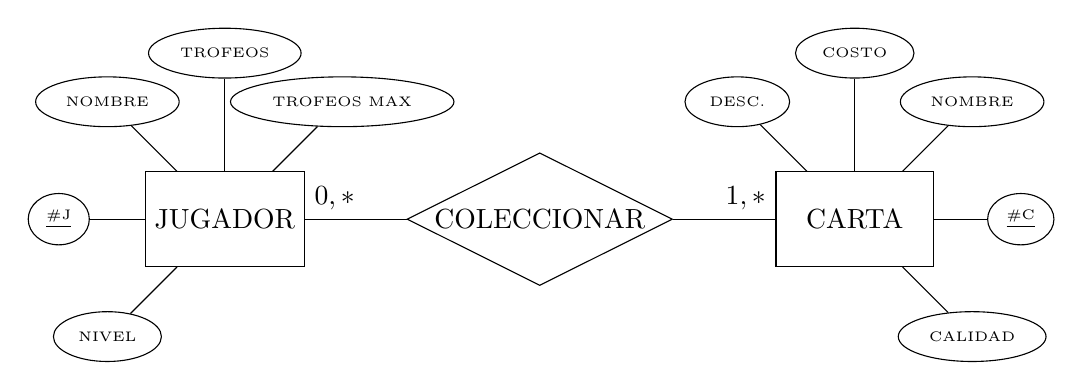
\begin{tikzpicture}[node distance=6em]
        \tikzstyle{every entity} = [minimum width=2cm, minimum height=1.2cm]
        \node[entity] (jugador) {JUGADOR}
            [sibling distance=3cm]
            child {node[attribute] [above right of=jugador] {\tiny TROFEOS MAX}}
            child {node[attribute] [above of=jugador] {\tiny TROFEOS}}
            child {node[attribute] [above left of=jugador] {\tiny NOMBRE}}
            child {node[attribute] [left of=jugador] {\underline{\tiny \#J}}}
            child {node[attribute] [below left of=jugador] {\tiny NIVEL}}
            ;
      
        \node[entity] (clan) at (8,0) {CARTA}
        [sibling distance=3cm]
        child {node[attribute] [right of=clan] {\underline{\tiny \#C}}}
        child {node[attribute] [above of=clan] {\tiny COSTO}}
        child {node[attribute] [above left of=clan] {\tiny DESC.}}
        child {node[attribute] [above right of=clan] {\tiny NOMBRE}}
        child {node[attribute] [below right of=clan] {\tiny CALIDAD}};
        
      
        \node[relationship,aspect=2] (pertenecer) at (4,0) {COLECCIONAR};
        \draw (pertenecer.east) -- (clan.west) node[above left] {$1,\ast$};
        \draw (pertenecer.west) -- (jugador.east) node[above right] {$0,\ast$};
    \end{tikzpicture}
\end{frame}




\begin{frame}{\'Algebra relacional}

    \begin{block}{Consultas}
        \begin{enumerate}
            \item<2-> Obtener el nombre de todos los jugadores cuyo nivel es al menos 10.
            \onslide<3->{$$r := \pi_{\text{\#J, Nombre}} (\text{Jugador}\,\sigma\, (\text{Nivel} \geq 10))$$}
            \item<4-> Obtener el nombre de todas las cartas cuya calidad sea \'epica.
            \onslide<5->{$$r := \pi_{\text{\#C, Nombre}} (\text{Carta}\,\sigma\, (\text{Calidad} = \text{"\'Epica"}))$$}
        \end{enumerate}
    \end{block}

\end{frame}


% \begin{frame}{\'Algebra relacional}

%     \begin{block}{Consultas}
%         \begin{enumerate}
%             \item Obtener el nombre de todos los jugadores cuyo nivel es al menos 10.
%             $$\pi_{\text{\#J, Nombre}} (\text{Jugador}\,\sigma\, (\text{Nivel} >= 10))$$ 
%             \item Obtener el nombre de todas las cartas cuya calidad sea \'epica.
%             $$\pi_{\text{\#C, Nombre}} (\text{Carta}\,\sigma\, (\text{Calidad} = \text{\'Epica}))$$
%         \end{enumerate}
%     \end{block}

% \end{frame}


\begin{frame}{\'Algebra relacional}

    \begin{block}{Consultas}
        \begin{enumerate}
            \setcounter{enumi}{2}
            \item Obtener el nombre de todos los jugadores que tienen la carta con identificador 2.
            $$ r_1 = \pi_{\text{\#J}, \text{Nombre}}((\text{Jugador} \Join \text{Coleccionar})\,\sigma\,(\text{\#C}=2)) $$
            $$ r_2 = \pi_{\text{\#J}, \text{Nombre}}(\text{Jugador} \Join (\text{Coleccionar}\,\sigma\,(\text{\#C}=2))) $$
        \end{enumerate}
        \vspace{5mm}

        \centering
        \large ¿Cu\'al es mejor?
        
        
    \end{block}
\end{frame}


\begin{frame}{El problema del \'algebra relacional}

   
    $$ \pi_{\text{\#J}, \text{Nombre}}((\text{Jugador} \Join \text{Coleccionar})\,\sigma\,(\text{\#C}=2)) $$

    \begin{block}{¿En qu\'e orden se ejecutan las operaciones?}
        \onslide<2->{
        \begin{enumerate}
            \item $\text{Jugador} \Join \text{Coleccionar}$\hspace{4mm} \onslide<3->{$O(|\text{Jugador}| \times |\text{Coleccionar}|)$}
            \item $(\text{Jugador} \Join \text{Coleccionar})\,\sigma\,(\text{\#C} = 2)$\hspace{4mm} \onslide<4->{$O(|\text{Coleccionar}|)$}
            \item $\pi_{\text{\#J}, \text{Nombre}}((\text{Jugador} \Join \text{Coleccionar})\,\sigma\,(\text{\#C}=2))$ \hspace{4mm} \onslide<5->{$O(|\text{Jugador}|)$}
        \end{enumerate}
        }

        \begin{center}
            \onslide<6->{
            \vspace{5mm}
            $
            O(|\text{Jugador}| \times |\text{Coleccionar}| + |\text{Coleccionar}| + |\text{Jugador}|)
            $
            }
            
            \onslide<7>{
            \vspace{2mm}
            $
            = O(|\text{Jugador}|^2 \times |\text{Carta}| + |\text{Coleccionar}| + |\text{Jugador}|)
            $\\[2mm]
            dado que $|\text{Coleccionar}| = O(|\text{Jugador}| \times |\text{Carta}|)$
            }

    
        \end{center}
    \end{block}
         
    
\end{frame}


\begin{frame}{El problema del \'algebra relacional}

   
    $$ \pi_{\text{\#J}, \text{Nombre}}(\text{Jugador} \Join (\text{Coleccionar}\,\sigma\,(\text{\#C}=2))) $$

    \begin{block}{¿En qu\'e orden se ejecutan las operaciones?}
        \onslide<2->{
        \begin{enumerate}
            \item $\text{Coleccionar} \,\sigma\, (\text{\#C = 2})$\hspace{4mm} \onslide<3->{$O(|\text{Coleccionar}|)$}
            \item $\text{Jugador} \Join (\text{Coleccionar} \,\sigma\,(\text{\#C} = 2))$\hspace{4mm} \onslide<4->{$O(|\text{Jugador}|^2)$}
            \item $\pi_{\text{\#J}, \text{Nombre}}(\text{Jugador} \Join (\text{Coleccionar}\,\sigma\,(\text{\#C}=2)))$ \hspace{4mm} \onslide<5->{$O  (|\text{Jugador}|)$}
        \end{enumerate}
        }

        \onslide<6>{

            $$
            O( |\text{Jugador}|^2 + |\text{Coleccionar}| +|\text{Jugador}| )
            $$
        }
    \end{block}
         
    
\end{frame}


\begin{frame}{El caracter imperativo del \'algebra relacional}
    \centering
    \Large No permite que el usuario se abstraiga de la optimizaci\'on

\end{frame}

\begin{frame}{Lenguajes de consulta declarativo}

    \begin{block}{C\'alculo relacional}
        \begin{itemize}
            \item C\'alculo relacional de tuplas
            \item C\'alculo relacional de dominios
        \end{itemize}
    \end{block}

\end{frame}


\begin{frame}{C\'alculo relacional de tuplas}
    \begin{block}{Definici\'on}
        Una consulta en el c\'alculo relacional de tuplas se expresa
        de la forma:

        $$
            \{t \,|\, P(t)\}
        $$
        donde: \begin{itemize}
            \item $t$ es una variable que representa una tupla
            \item $P$ es una f\'ormula bien formada compuesta de \'atomos
        \end{itemize}
    \end{block}
\end{frame}






\begin{frame}{C\'alculo relacional de tuplas}

    \begin{block}{Consultas}
        \begin{enumerate}
            \item Obtener todos los jugadores cuyo nivel es al menos 10.
            \onslide<2->{$$\{t \,|\, t \in \text{Jugador} \land t[\text{Nivel}] \geq 10\}$$} 
            \item<3-> Obtener el nombre de todos los jugadores cuyo nivel es al menos 10.
            \onslide<4->{$$\{t \,|\, \exists\, j \in \text{Jugador}(t[\text{\#J}] = j[\text{\#J}] \land t[\text{Nombre}] = j[\text{Nombre}] \land j[\text{Nivel}] \geq 10)\}$$}
        \end{enumerate}
    \end{block}

\end{frame}


\begin{frame}{C\'alculo relacional de tuplas}
 
    \begin{block}{Consultas}
        \begin{enumerate}
            \setcounter{enumi}{2}
            \item Obtener el nombre de todos los jugadores que tienen la carta con identificador 2.
            \onslide<2>{

                \begin{scriptsize}
                    $$ \{t | \exists j \in \text{Jugador} (t[\text{\#J}] = j[\text{\#J}] \land  t[\text{Nombre} ]= j[\text{Nombre}] \land \exists c \in \text{Coleccionar} ( j[\text{\#J}] = c[\text{\#J}] \land c[\text{\#C}] = 2 ))\}$$
                    
                \end{scriptsize}
            }
                
            
        \end{enumerate}

        
        
    \end{block}

\end{frame}

\begin{frame}{C\'alculo relacional de dominios}
    \begin{block}{Definici\'on}
        Una consulta en el c\'alculo relacional de dominios se
        expresa de la forma
        $$
            \{<x_1,x_2,...,x_n\> | P(x_1,x_2,...,x_n)\}
        $$
        donde: \begin{itemize}
            \item $x_1,x_2,...,x_n$ son variables de dominio
            \item $P$ es una f\'ormula bien formada compuesta de \'atomos
        \end{itemize}
    \end{block}
\end{frame}


\begin{frame}{C\'alculo relacional de dominios}

    \begin{block}{Consultas}
        Sean las variables $a, b, c ,d ,e$ correspondientes a \#J, Nombre, Nivel, Trofeos, TrofeosMax en la relaci\'on Jugador.

        \begin{enumerate}
            \item Obtener todos los jugadores cuyo nivel es al menos 10.
            \onslide<2->{$$\{<a,b,c,d,e> \,|\,  <a,b,c,d,e> \in \text{Jugador} \land c \geq 10\}$$} 
            \item<3-> Obtener el nombre de todos los jugadores cuyo nivel es al menos 10.
            \onslide<4->{$$\{<a,b> \,|\, \exists c,d,e(<a,b,c,d,e> \in \text{Jugador} \land c \geq 10)\}$$}
        \end{enumerate}
    \end{block}

\end{frame}

\begin{frame}{C\'alculo relacional de dominios}
    
    \begin{block}{Consultas}
        Sean las variables $a, b, c ,d ,e$ correspondientes a \#J, Nombre, Nivel, Trofeos, TrofeosMax en la relaci\'on Jugador.
        Sea la variable $f$ correspondiente a \#C en la relaci\'on Coleccionar.
        \begin{enumerate}
            \item Obtener el nombre de todos los jugadores que tienen la carta con identificador 2.
            \onslide<2->{

                \begin{small}
                    $$\{<a,b> \,|\, \exists c,d,e(<a,b,c,d,e> \in \text{Jugador} \land \exists f(<a,f> \in Coleccionar \land f=2))\}$$ 
                    
                \end{small}
            }
                
            
        \end{enumerate}

        
        
    \end{block}

\end{frame}


\begin{frame}{Equivalencia entre lenguajes}
    \begin{block}{El teorema de Codd}
        \begin{itemize}
            \item Para toda expresi\'on $E$ del \'algebra
            relacional existe una consulta $Q$ del c\'alculo relacional
            tal que $E \equiv  Q$
            \item Para toda consulta $Q$ del c\'alculo
            relacional existe una expresi\'on algebraica $E$ 
            tal que $Q \equiv  E$
        \end{itemize}

        El c\'alculo relacional es un lenguaje relacional completo
    \end{block}

    \onslide<2->{

        \begin{block}{Optimizaci\'on de consultas}
            Transformar una consulta $Q$ del c\'alculo relacional en una expresi\'on $E$ del \'algebra relacional.
        \end{block}
    }
\end{frame}


\begin{frame}
    \vspace{10mm}

    \centering
    \begin{Huge}
        
        \textcolor{blue3}{Turing completo vs Relacional completo}
    \end{Huge}

    \onslide<2>{

        \begin{columns}[T]
            \begin{column}{0.48\linewidth}
                \begin{itemize}
                    \item Mayor expresividad
                    \item No puede ser optimizado para el caso general de forma autom\'atica.
                \end{itemize}
            \end{column}
    
            \begin{column}{0.48\linewidth}
                \begin{itemize}
                    \item Menor expresividad
                    \item Puede ser optimizado para el caso general de forma autom\'atica.
                \end{itemize}
            \end{column}
            
        \end{columns}
    }
\end{frame}



    
\begin{frame}{Entonces...}

    \begin{columns}[T]
        \begin{column}{0.4\linewidth}
            \vspace{3.3cm}

            \Huge ... alguna duda?
        \end{column}
        \begin{column}{0.58\linewidth}
            
            
\includegraphics[height=0.8\textheight, width=\linewidth]{img/eval.jpg}
        \end{column}
        
    \end{columns}
    
\end{frame}

\end{document}
